% 第1節 場合の数
\section{場合の数}
\subsection{集合の要素の個数}
% 割愛

\subsection{場合の数}
% 割愛

\subsection{順列}
% 順列
\begin{definitionbox}[def:順列]{\textbf{順列}}
    いくつかのものを順に1列に並べるとき, その並びの1つ1つを \textbf{順列} という.

    一般に, \uwave{異なる $n$ 個のものから異なる $r$ 個を取り出して}並べる順列を
    \begin{center}
        $\bm{n}$\textbf{個から}$\bm{r}$\textbf{個取る順列}
    \end{center}
    といい, その総数を $_{\bm{n}}\mathbf{P}_{\bm{r}}$ $^{*}$ で表す.
\end{definitionbox}

\begin{theorembox}[thm:順列の総数①]{\textbf{順列の総数① $_{\bm{n}}\mathbf{P}_{\bm{r}}$}}
    $n$ 個から $r$ 個取る順列の総数 $_{n}\mathrm{P}_{r}$ は次の式で表される.

    \begin{align}
        _{\bm{n}}\mathbf{P}_{\bm{r}} = \bm{n \cdot (n-1) \cdot (n-2) \cdots \cdots (n-r+1)}
        \label{eq:順列の総数①}
    \end{align}
\end{theorembox}
\newpage

% 練習14
\begin{exercise}[【教p.24 練習14】]
    次のものの総数を求めよ.
    \begin{enumerate}
        \item 10人の生徒から3人を選んで1列に並べるときの並び順
        \item 7個の数字 1, 2, 3, 4, 5, 6, 7 のうちの異なる4個を並べて作る4桁の整数
    \end{enumerate}
\end{exercise}

    \begin{proof}\mbox{}\\
        (1) 10人の生徒から3人を選んで1列に並べる順列の総数であるから,

        \begin{alignanswer*}
            {}_{10}\mathrm{P}_{3} &= 10 \cdot 9 \cdot 8 \\
                                &= 720 \quad \text{(通り)}
        \end{alignanswer*}
    \end{proof}
    \vspace{1em}

    \begin{proof}\mbox{}\\
        (2) 7個の数字から4個を選んで並べる順列の総数であるから,

        \begin{alignanswer*}
            {}_{7}\mathrm{P}_{4} &= 7 \cdot 6 \cdot 5 \cdot 4 \\
                            &= 840 \quad \text{(通り)}
        \end{alignanswer*}
    \end{proof}
\newpage

順列の総数 ${}_n\mathrm{P}_r$ の式で, 特に $r = n$ のときは等式

\begin{align*}
    _{n}\mathrm{P}_{n} = n(n-1)(n-2) \cdots \cdots 3 \cdot 2 \cdot 1 \tag{*}
\end{align*}

が得られる.

% 階乗
\begin{definitionbox}[def:階乗]{\textbf{階乗}}
    $(*)$ の右辺は, $1$ から $n$ までのすべての自然数の積である.

    これを $n$ の \textbf{階乗} といい, $\bm{n!}$ で表す.
\end{definitionbox}

\begin{theorembox}[thm:階乗]{\textbf{階乗}}
    Definition\ref{def:階乗} より, $n$ の階乗 $n!$ は次の式で表される.

    \begin{align}
        _{\bm{n}}\mathbf{P}_{\bm{r}} \bm{=} \bm{n!} \bm{=} \bm{n (n-1) (n-2) \cdots \cdots 3 \cdot 2 \cdot 1}
        \label{eq:階乗}
    \end{align}
\end{theorembox}
\vspace{1em}

Definition\ref{def:順列}より, 一般に, 次のことがいえる.

\[\textbf{異なる} \bm{n} \textbf{個のものすべてを並べる順列の総数は}\;\; \bm{n!} \;\;\textbf{である}\]

また, 順列の総数 ${}_n\mathrm{P}_r$ の式で, $r < n$ のときについて考える.
\vspace{1em}

% 証明
\begin{samepage}
\begin{proof}\mbox{}\\
    \begin{align*}
        _{n}\mathrm{P}_{r} &= n (n-1) (n-2) \cdots \cdots 3 \cdot 2 \cdot 1\\
                        &= \dfrac{\,n (n-1) (n-2) \cdots \cdots (n-r+1) \bm{(n - r) \cdots \cdots 3 \cdot 2 \cdot 1}\,}
                        {\,\bm{(n - r) \cdots \cdots 3 \cdot 2 \cdot 1}\,} \\
                        &= \dfrac{\,\bm{n!}\,}{\,\bm{(n - r)!}\,}
    \end{align*}
    \vspace{-5\baselineskip}%  この証明環境だけ空行を追加しない(□の前に配置)
\end{proof}
\vspace{1em}%  □と次の定理環境の間に適切な間隔を確保
\end{samepage}

\begin{theorembox}[thm:順列の総数②]{\textbf{順列の総数② $_{\bm{n}}\mathbf{P}_{\bm{r}}$}}

    \begin{align}
        _{\bm{n}}\mathbf{P}_{\bm{r}} \bm{=} \dfrac{\,\bm{n!}\,}{\,\bm{(n-r)}\bm{!}\,}
        \label{eq:順列の総数②}
    \end{align}
\end{theorembox}
\vspace{1em}

Theorem\ref{thm:順列の総数②}が $r = 0, r = n$ のときも成り立つように, ${}_{\bm{n}}\mathbf{P}_{\bm{0}} \bm{= 1}$ , $\bm{0! = 1}$ と定めることとする.


\vfill

\noindent
\rule{\textwidth}{0.4pt}

\noindent
$^{*}$ ${}_n\mathrm{P}_r$ の P は 順列を意味するPermutation の頭文字である.\\

\newpage

% 練習16
\begin{exercise}[【教p.25 練習16】]
    12色の色鉛筆がある. A, B, C の3つの文字を, すべて異なる色で塗り分けるとき, 塗り方は何通りあるか.
\end{exercise}

    \begin{proof}\mbox{}\\
        12色の色鉛筆から3色を選んで1列に並べ左の色から順に, A, B, C と塗り分けると考えれば良いため,

        \begin{alignanswer*}
            {}_{12}\mathrm{P}_{3} &= 12 \cdot 11 \cdot 10 \\
                                &= 1320 \quad \text{(通り)}
        \end{alignanswer*}
    \end{proof}
    \vspace{1em}

% テクニック
% 応用例題4
    \begin{example}[【教p.26 応用例題4】]
        大人4人と子ども3人が1列に並ぶとき, 次のような並び方は何通りあるか.
        \begin{enumerate}
            \item 両端が大人である.
            \item 子どもが3人続いて並ぶ.
        \end{enumerate}
    \end{example}

    \begin{techniquebox}[tech:83]{\textbf{隣り合うものは合体させて, 隣り合わないものは最後に挿入しよう!}}
        「隣り合う」という条件が与えられれば, 合体させたものについても, 自身の \textbf{階乗通り} の合体方法があることに注意したい.

        一方, 「隣り合わない」という条件が与えられれば, それを \textbf{間または両端} に挿入することを考えよう!
    \end{techniquebox}

    \begin{proof}\mbox{}\\
        (1) 両端の大人の並び方は,  $\answermath{{}_{4}\mathrm{P}_{2}}$ 通りある.

        そのどの場合に対しても, 間に並ぶ残りの5人の並び方は, $\answermath{5!}$ 通りある.

        よって, 並び方の総数は, \fitblankbf[積の法則]{8} により

        \begin{alignanswer*}
            {}_{4}\mathrm{P}_{2} \times 5! &= 12 \times 120 \\
                                &= 1440 \quad \text{(通り)}
        \end{alignanswer*}
    \end{proof}

    \begin{proof}\mbox{}\\
        (2) 子ども3人をひとまとめにする.

        大人4人とひとまとめにした子ども4人の並び方は, $\answermath{5!}$ 通りある.
        そのどの場合に対しても, ひとまとめにした子ども3人の並び方は, $\answermath{3!}$ 通りある.

        よって, 並び方の総数は, \fitblankbf[積の法則]{8} により

        \begin{alignanswer*}
            5! \times 3! &= 5 \cdot 4 \cdot 3 \cdot 2 \cdot 1 \times 3 \cdot 2 \cdot 1 \\
                                &= 720 \quad \text{(通り)}
        \end{alignanswer*}
    \end{proof}
    \vspace{1em}
\newpage

% 応用例題5
\begin{example}[【教p.27 応用例題5】]
    6個の数字 0, 1, 2, 3, 4, 5 のうちの異なる4個を並べて,4桁の整数を作るとき,次のような整数は何個作れるか。
    \begin{enumerate}
        \item 4桁の整数
        \item 4桁の奇数
    \end{enumerate}
\end{example}
\vspace{-1em}%  例題環境後の空行を減らす

\begin{techniquebox}[tech:79]{\textbf{場合の数・確率の問題は, いかに状況を整理するかを考えよ!}}
    「どのように場合分けすればよいか」「この条件は, 要はどういうことなのか」などを, \textbf{実験を通して} 考えよう.

    1つの方針として, \textbf{制限のあるもの} から考える, というものがある.
\end{techniquebox}
\vspace{-0.5em}%  テクニックボックス後の空行を減らす

\begin{proof}\mbox{}\\
    (1)千の位は, 0以外の数字 1, 2, 3, 4, 5 のどれかであるから, その選び方は $\answermath{5}$ 通りある.

    そのどの場合に対しても, 百, 十, 一の位には, 残りの5個の数字から3個取って並べるから,
    その並び方は $\answermath{_{5}\mathrm{P}_{3}}$ 通りある.

    よって, 求める個数は, 積の法則により

    \begin{alignanswer*}
        5 \times {}_{5}\mathrm{P}_{3} &= 5 \times 5 \cdot 4 \cdot 3 \\
                                &= 300 \quad \text{(個)}
    \end{alignanswer*}
    \vspace{-3\baselineskip}%  この証明環境の空行を減らす
\end{proof}
\vspace{-0.5em}%  証明環境間の空行を減らす

\begin{proof}\mbox{}\\
    (2) 一の位は, 数字 1, 3, 5 のどれかであるから, その選び方は $\answermath{3}$ 通りある.

    そのどの場合に対しても, 千の位は, 0 と一の位の数字以外の4個の数字のどれかであるから, その選び方は $\answermath{4}$ 通りある.

    さらに, 百, 十の位には, 残りの4個の数字から2個取って並べるから, その \uwave{並べ方}は $\answermath{_{4}\mathrm{P}_{2}}$ 通りある.

    よって, 求める個数は, 積の法則により

    \begin{alignanswer*}
        3 \times 4 \times {}_{4}\mathrm{P}_{2} &= 3 \times 4 \times 4 \cdot 3 \\
                                &= 144 \quad \text{(個)}
    \end{alignanswer*}
    \vspace{-3\baselineskip}%  この証明環境の空行を減らす
\end{proof}
\newpage

\begin{definitionbox}[def:円順列]{\textbf{円順列}}
    いくつかのものを円形に並べる順列を \textbf{円順列} という.

    円順列では, \uwave{回転して並びが同じになるものは同じ並び方とみなす}.
\end{definitionbox}

% テクニック

\begin{theorembox}[thm:円順列の総数]{\textbf{円順列の総数}}
    異なる $n$ 個のものの円順列の総数について, 次のことがいえる.

    \begin{align}
        \dfrac{\,_{\bm{n}}\mathbf{P}_{\bm{n}}\,}{\,\bm{n}\,} \bm{= (n-1)!}
        \label{eq:円順列の総数}
    \end{align}
\end{theorembox}

% 練習19
\begin{exercise}[【教p.29 練習19】]
    色の異なる6個の玉を円形に並べて置くとき, 並べ方の総数を求めよ.
\end{exercise}

\begin{techniquebox}[tech:86]{\textbf{円順列は, 1箇所を固定して考えよ!}}
    ある1箇所を固定してしまえば, 残りの箇所は \textbf{区別できるようになる} ため, 今までの順列の問題と同様に処理することができる.
\end{techniquebox}

    \begin{proof}\mbox{}\\
        \begin{alignanswer*}
            (6-1)! &= 5! \\
                    &= 120 \quad \text{(通り)}
        \end{alignanswer*}
    \end{proof}
\newpage

% 応用例題6
\begin{example}[【教p.29 応用例題6】]
        先生4人と生徒4人が輪の形に並ぶとき, 先生と生徒が交互に並ぶような並び方は何通りあるか。
    \end{example}

    \begin{proof}\mbox{}\\
        先生が円形に並んで, 間に生徒が並んでいくと考えればよい. 先生が円形に並んでから特定の生徒を基準にすると,
        間に入る生徒の並び方は, 1列に並ぶ順列と考えることができる.

        先生4人の円順列の総数は, $\answermath{(4-1)!}$ 通りある.

        そのどの場合に対しても, 生徒4人が先生の間に1人ずつ並ぶ方法は, $\answermath{4!}$ 通りある.

        よって, 求める並び方の総数は, 積の法則により

        \begin{alignanswer*}
            (4-1)! \times 4! &= 3 \cdot 2 \cdot 1 \times 4 \cdot 3 \cdot 2 \cdot 1 \\
                                &= 144 \quad \text{(通り)}
        \end{alignanswer*}
    \end{proof}
\newpage

% じゅず順列
% \vspace{1em}

ここまでは, 異なるものだけを並べる順列を考えてきた. ここでは, 同じものを繰り返し使うことを許した場合の順列を考えてみよう.

% 重複順列
\begin{definitionbox}[def:重複順列]{\textbf{重複順列}}
    一般に, \uwave{異なる $n$ 種類のものから重複を許して $r$ 個取って} 並べる順列を
    \bm{$n$} \textbf{個から} \bm{$r$} \textbf{個取る重複順列} という.

    重複順列では, $r \leqq n$ とは限らず, $r > n$ であってもよい.
\end{definitionbox}

\begin{theorembox}[thm:重複順列の総数]{\textbf{重複順列の総数}}
    重複順列の総数について, 次のことがいえる.

    \begin{align}
        n \text{個から} r \text{個取る重複順列の総数は} \qquad \bm{n^r}
        \label{eq:重複順列の総数}
    \end{align}
\end{theorembox}

% 練習22
\begin{exercise}[【教p.30 練習22】]
    4個の文字 a, b, c, d を, 重複を許して次の個数だけ1列に並べるとき, 何通りの文字列が作れるか。
    \begin{enumerate}
        \item 2個
        \item 3個
    \end{enumerate}
\end{exercise}
\vspace{-1em}%  練習問題環境後の空行を減らす

\begin{proof}\mbox{}\\
    (1) 4個から2個取る重複順列であるから,

    \begin{alignanswer*}
        4^2 &= 16 \quad \text{(通り)}
    \end{alignanswer*}
    \vspace{-3\baselineskip}%  この証明環境の空行を減らす
\end{proof}
\vspace{-0.5em}%  証明環境間の空行を減らす

\begin{proof}\mbox{}\\
    (2) 4個から3個取る重複順列であるから,

    \begin{alignanswer*}
        4^3 &= 64 \quad \text{(通り)}
    \end{alignanswer*}
    \vspace{-3\baselineskip}%  この証明環境の空行を減らす
\end{proof}
\newpage

\subsection{組合せ}

% 組合せ
\begin{definitionbox}[def:組合せ]{\textbf{組合せ}}
    一般に, \uwave{異なる $n$ 個のものから異なる $r$ 個を取り出して} 作る組合せを
    \begin{center}
        $\bm{n}$\textbf{個から}$\bm{r}$\textbf{個取る組合せ}
    \end{center}
    といい, その総数を $_{\bm{n}}\mathbf{C}_{\bm{r}}$ $^{*}$ で表す. ただし, $r \leqq n$ とする.
\end{definitionbox}
\vspace{1em}

ここで, Permutation と Combination の違いを確認しておこう.

まずは, 日本語の意味の違いから. Permutation は「\textbf{順列}」, Combination は「\textbf{組合せ}」である.

次に, 数学的な視点から, Permutation と Combination の違いを考えてみよう.

% 証明
例えば, 5個から3個取る組合せの総数は ${}_5\mathrm{C}_{3}$ で表され, それは \uwave{\text{10 (通り)}} であるが, これを順列の総数から考えてみよう.

5個から3個取る順列の総数 ${}_5\mathrm{P}_{3}$ は, 次のように考えることもできる.

\[\text{5個から3個取る組合せを作り, }(\answermath{{}_5\mathrm{C}_{3}} \text{ 通り})\]
\[\text{取り出した3個すべてを1列に並べる}(\answermath{3!} \text{ 通り})\]

よって, 積の法則により, 次の等式が成り立つ.

\[\answermath{{}_5\mathrm{C}_{3}} \times \answermath{3!} = \answermath{{}_5\mathrm{P}_{3}}\]

したがって, $\answermath{{}_5\mathrm{C}_{3}}  = \dfrac{\,\answermath{{}_5\mathrm{P}_{3}\,}}{\,\answermath{3!\,}}
= \dfrac{\,5 \cdot 4 \cdot 3\,}{\,3 \cdot 2 \cdot 1\,} = \uwave{10}$ \uwave{(通り)}
\vspace{1em}

これを一般化したものを次に示す.

\begin{theorembox}[thm:組合せの総数]{\textbf{組合せの総数 $_{\bm{n}}\mathbf{C}_{\bm{r}}$}}
    $n$ 個から $r$ 個取る組合せの総数 $_{n}\mathrm{C}_{r}$ は次の式で表される.

    \begin{align}
        {}_{\bm{n}}\mathrm{C}_{\bm{r}} \bm{=} \dfrac{\,{}_{\bm{n}}\mathrm{P}_{\bm{r}}\,}{\,\bm{r!}\,} \bm{=}
        \dfrac{\,\bm{n(n-1)(n-2)\cdots\cdots(n-r+1)}\,}{\,\bm{r(r-1)(r-2)\cdots\cdots \cdot 3 \cdot 2 \cdot 1}\,}
        \label{eq:組合せの総数}
    \end{align}
\end{theorembox}
\vspace{1em}

Theorem\ref{eq:組合せの総数}において, 特に ${}_n\mathrm{C}_1 = n$ , ${}_n\mathrm{C}_n = 1$ である.

また, 式\ref{eq:順列の総数②}より,

\begin{align*}
    {}_n\mathrm{C}_r &= \dfrac{\,{}_n\mathrm{P}_r\,}{\,r!\,} && \text{( $\because$ 式\ref{eq:組合せの総数})}\\
                    &=  \dfrac{\dfrac{\,n!\,}{\,(n-r)!\,}}{\;r!\;} && \text{( $\because$ 式\ref{eq:順列の総数②})}\\
                    &= \answermath{\dfrac{\;n!\;}{\;r!\;(n - r)!\;}}
\end{align*}
\vspace{1em}

と表すこともできる. ただし, ${}_n\mathrm{C}_0 = 1$ と定めることとする.
\newpage

% 練習24
\begin{exercise}[【教p.33 練習24】]
    次のような選び方の総数を求めよ.
    \begin{enumerate}
        \item 8人から2人を選ぶ
        \item 7色から4色を選ぶ
    \end{enumerate}
\end{exercise}

    \begin{proof}\mbox{}\\
        (1) 8個から2個取る組合せであるから,

        \begin{alignanswer*}
            _{8}\mathrm{C}_{2} &= \dfrac{\,8 \cdot 7\,}{\,2 \cdot 1\,} \\
                                &= 28 \quad \text{(通り)}
        \end{alignanswer*}
    \end{proof}

    \begin{proof}\mbox{}\\
        (2) 7個から4個取る組合せであるから,

        \begin{alignanswer*}
            _{7}\mathrm{C}_{4} &= \dfrac{\,7 \cdot 6 \cdot 5 \cdot 4\,}{\,4 \cdot 3 \cdot 2 \cdot 1\,} \\
                                &= 35 \quad \text{(通り)}
        \end{alignanswer*}
    \end{proof}
\newpage

練習24(1)において, 8人から2人選ぶことは, 選ばない6人を選ぶことと同じである。

よって, 次の等式が成り立つ。

\[{}_{8}\mathrm{C}_{2} = \answermath{{}_{8}\mathrm{C}_{6}}\]

これを一般化したものを次に示す.

\begin{theorembox}[thm:]{\textbf{$_{\bm{n}}\mathbf{C}_{\bm{r}}$ の性質}}
    一般に, $n$ 個から $r$ 個取る組合せの総数は, $n$ 個から $(n-r)$ 個取る組合わせの総数に等しい.
    すなわち, 次の等式が成り立つ.
    \begin{align}
        {}_{\bm{n}}\mathbf{C}_{\bm{r}} \bm{=} {}_{\bm{n}}\mathbf{C}_{\bm{n-r}}
    \end{align}
\end{theorembox}

% 練習26
\begin{exercise}[【教p.34 練習26】]
    正六角形について, 次の数を求めよ.
    \begin{enumerate}
        \item 3個の頂点を結んでできる三角形の個数
        \item 2個の頂点を結ぶ線分の本数
    \end{enumerate}
\end{exercise}
\vspace{-1em}%  練習問題環境後の空行を減らす

    \begin{proof}\mbox{}\\
        (1) 6個の頂点はどの3点も一直線上にないから, 3個の点を1組決めると三角形を1個作ることができる.

        \begin{alignanswer*}
            _{6}\mathrm{C}_{3} &= \dfrac{\answermath{6 \cdot 5 \cdot 4}}{\answermath{3 \cdot 2 \cdot 1}} \\
                                &= 20 \quad \text{(個)}
        \end{alignanswer*}
        \vspace{-3\baselineskip}%  この証明環境の空行を減らす
    \end{proof}
    \vspace{-0.5em}%  証明環境間の空行を減らす

    \begin{proof}\mbox{}\\
        (2) 6個の頂点それぞれに対して, 相方の点を1個決めると2個の頂点を結ぶ線分を1本作ることができる.

        \begin{alignanswer*}
            _{6}\mathrm{C}_{2} &= \dfrac{\answermath{6 \cdot 5}}{\answermath{2 \cdot 1}} \\
                                &= 15 \quad \text{(本)}
        \end{alignanswer*}
        \vspace{-3\baselineskip}%  この証明環境の空行を減らす
    \end{proof}
    \vspace{-0.5em}%  証明環境と例題環境間の空行を減らす

% 応用例題7
\begin{example}[【教p.35 応用例題7】]
    大人6人, 子ども4人の中から, 5人を選ぶとき, 次のような選び方は何通りあるか.
    \begin{enumerate}
        \item 大人3人と子ども2人を選ぶ.
        \item 子どもが少なくとも1人は含まれるように選ぶ.
    \end{enumerate}
\end{example}
\vspace{-1.5em}%  例題環境後の空行をさらに減らす

\begin{techniquebox}[tech:80]{\textbf{場合の数・確率の問題では, 常に余事象を疑え!}}
    \textbf{「少なくとも〜」というキーワードがあれば}, 余事象は限られるため容易に疑える.

    しかし, \textbf{そのようなキーワードがなくとも余事象を考えたほうが楽な場合も多い} ため, 余事象を疑うことを習慣化しよう.
\end{techniquebox}
\vspace{-1em}%  テクニックボックス後の空行をさらに減らす

\begin{proof}\mbox{}\\
    (1) 大人と子どもを別々に選び, 積の法則を用いて求めたい.

    大人3人の選び方は, $\answermath{{}_{6}\mathrm{C}_{3}}$ 通りある.

    そのどの場合に対しても, 子ども2人の選び方は, $\answermath{{}_{4}\mathrm{C}_{2}}$ 通りある.

    よって, 求める選び方の総数は, 積の法則により

    \begin{alignanswer*}
        {}_{6}\mathrm{C}_{3} \times {}_{4}\mathrm{C}_{2} &= \dfrac{\answermath{6 \cdot 5 \cdot 4}}{\answermath{3 \cdot 2 \cdot 1}}
        \times \dfrac{\answermath{4 \cdot 3}}{\answermath{2 \cdot 1}} \\
                                &= 120 \quad \text{(通り)}
    \end{alignanswer*}
    \vspace{-4\baselineskip}%  この証明環境の空行をさらに減らす
\end{proof}
\vspace{-1em}%  証明環境間の空行をさらに減らす

\begin{proof}\mbox{}\\
    (2) 「少なくとも1人」は「1人以上」という意味である. したがって, 余事象が「 \answertext{\textbf{0人}} 」と限定されるためこれを利用する.

    10人から5人の選び方は, $\answermath{{}_{10}\mathrm{C}_{5}}$ 通りある.

    子どもが1人も選ばれず, 5人とも大人となる選び方は, $\answermath{{}_{6}\mathrm{C}_{5}}$ 通りある.

    よって, 求める選び方の総数は

    \begin{alignanswer*}
        {}_{10}\mathrm{C}_{5} - {}_{6}\mathrm{C}_{5} &= {}_{10}\mathrm{C}_{5} - {}_{6}\mathrm{C}_{1}\\
                        &= \dfrac{\answermath{10 \cdot 9 \cdot 8 \cdot 7 \cdot 6}}{\answermath{5 \cdot 4 \cdot 3 \cdot 2 \cdot 1}} - 6\\
                                &= 252 - 6 \\
                                &= 246 \quad \text{(通り)}
    \end{alignanswer*}
    \vspace{-4\baselineskip}%  この証明環境の空行をさらに減らす
\end{proof}
\newpage

% 応用例題8
\begin{example}[【教p.36 応用例題8】]
    6人を次のように分けるとき, 分け方は何通りあるか.
    \begin{enumerate}
        \item A, B, C の3つの部屋に, 2人ずつ分ける.
        \item 2人ずつの3つの部屋に分ける.
    \end{enumerate}
\end{example}
\vspace{-1.5em}%  例題環境後の空行を減らす

\begin{proof}\mbox{}\\
    (1)部屋Aの2人の選び方は $\answermath{{}_{6}\mathrm{C}_{2}}$ 通りある.

    部屋Bの2人の選び方は残りの4人から選ぶので $\answermath{{}_{4}\mathrm{C}_{2}}$ 通り,

    部屋A, B の人が決まれば, 残りの部屋Cの2人は決まる.

    よって, 分け方の総数は, 積の法則により

    \begin{alignanswer*}
        {}_{6}\mathrm{C}_{2} \times {}_{4}\mathrm{C}_{2} &= \dfrac{\answermath{6 \cdot 5}}{\answermath{2 \cdot 1}}
        \times \dfrac{\answermath{4 \cdot 3}}{\answermath{2 \cdot 1}} \\
                                &= 90 \quad \text{(通り)}
    \end{alignanswer*}
    \vspace{-4\baselineskip}%  この証明環境の空行を減らす
\end{proof}
\vspace{-1em}%  証明環境とテクニックボックス間の空行を減らす

\begin{techniquebox}[tech:82]{\textbf{区別できないものを含む場合は, あえて異なるものとして区別して, 重複度で割る方法を疑え!}}
    \textbf{区別できないものをあえて区別して考えた上で, 重複度で割ること} で, 場合の数を求める手法が有効なことも多い.

    なお, 問題によっては \textbf{重複度の異なるものが混在している場合もある} ので, 検討は丁寧に行うことに注意したい.
\end{techniquebox}
\vspace{-1em}%  テクニックボックス後の空行を減らす

\begin{proof}\mbox{}\\
    (2) 本問と前問の違いは, 部屋に名前がついているかいないか, すなわち, それぞれの組を区別できるかできないかである.
    (人数が違えば, それは区別できる.)

    例えば, 1つの組分け \{a, b\}, \{c, d\}, \{e, f\} において, この3つの組にA, B, C の名前をつけるとすると,
    $\answermath{3!}$ 通りのつけ方がある. よって, 本問の総数を求めるには, 前問の答えを $\answermath{3!}$ で割ればよい.

    \vspace{0.5em}%  証明環境内の空行を減らす

    (1)で, A, B, C の区別をなくすと, $\answermath{3!}$ 通りずつ同じ組み分けができる. $^{*}$

    よって, 分け方の総数は

    \begin{alignanswer*}
        \dfrac{\,90\,}{\,3!\,} &= \dfrac{\,90\,}{\,6\,} \\
                        &= 15 \quad \text{(通り)}
    \end{alignanswer*}
    \vspace{-4\baselineskip}%  この証明環境の空行を減らす
\end{proof}
\newpage

ここで, もう一度 Permutation と Combination の違いを復習しておこう.

まずは, 日本語の意味の違いから. Permutation は「順列」, Combination は「組合せ」である.
したがって, 順列の総数を求めたいときは Permutation を, 組合せの総数を求めたいときは Combination を使ってきたと思う.

しかし, ここからは「順列」の総数を求めるのに, 「組合せ」Combination を利用できる場合があるということを覚えておこう.
これが, Permutation と Combination を混同させる原因の一つである.

\begin{theorembox}[thm:同じものを含む順列の総数]{\textbf{同じものを含む順列の総数}}
    $a$ が $p$ 個, $b$ が $q$ 個, $c$ が $r$ 個あるとき, それら全部を1列に並べる順列の総数は

    \begin{align}
        {}_{n}\mathrm{C}_{p} \times {}_{n-p}\mathrm{C}_{q} = \dfrac{\,\bm{n!}\,}{\,\bm{p!\;q!\;r!}\,} \qquad \qquad
        \text{ただし} \qquad p + q + r = n
        \label{eq:同じものを含む順列の総数}
    \end{align}
\end{theorembox}
\vspace{-1em}%  定理環境後の空行をさらに減らす

$r = 0$ のときは, ${}_{n-p}\mathrm{C}_{q} = 1$ であり, 順列の総数は $\dfrac{\,n!\,}{\,p!\;q!\,}$ である.

% 例題7
\begin{example}[【教p.38 例題7】]
    9個の数字 1, 1, 1, 1, 2, 2, 2, 3, 3, の全部を使って, 9桁の整数を作るとき, 何個の整数が作れるか.
\end{example}
\vspace{-1.5em}%  例題環境後の空行を減らす

\begin{proof}\mbox{}\\
    1 が4個, 2 が3個, 3 が2個あり, これらを1列に並べるから

    \begin{alignanswer*}
        \dfrac{\,9!\,}{\,4! \cdot 3! \cdot 2!\,} &= \dfrac{\,9 \cdot 8 \cdot 7 \cdot 6 \cdot 5 \cdot 4 \cdot 3 \cdot 2 \cdot 1\,}
        {\,4 \cdot 3 \cdot 2 \cdot 1 \times 3 \cdot 2 \cdot 1 \times 2 \cdot 1\,} \\
                                &= 1260 \quad \text{(個)}
    \end{alignanswer*}
    \vspace{-4\baselineskip}%  この証明環境の空行を減らす
\end{proof}
\vspace{-1em}%  証明環境と練習問題環境間の空行をさらに減らす

% 練習29
\begin{exercise}[【教p.39 練習29】]
    BANANA の6文字すべて使って文字列を作るとき, 何通りの文字列が作れるか.
\end{exercise}
\vspace{-1em}%  練習問題環境後の空行を減らす

    \begin{proof}\mbox{}\\
        BANANA の6文字は, B が1個, A が3個, N が2個あり, これらを1列に並べるから

        \begin{alignanswer*}
            \dfrac{\,6!\,}{\,3! \cdot 2!\,} &= \dfrac{\,6 \cdot 5 \cdot 4 \cdot 3 \cdot 2 \cdot 1\,}
            {\,3 \cdot 2 \cdot 1 \times 2 \cdot 1\,} \\
                                &= 60 \quad \text{(通り)}
        \end{alignanswer*}
        \vspace{-4\baselineskip}%  この証明環境の空行を減らす
    \end{proof}

% 応用例題9
\begin{example}[【教p.39 応用例題9】]
    \begin{minipage}{0.6\textwidth}
        右の図は, ある地域の道を直線で示したものである. 交差点Aから交差点Bまで遠回りしないで行く
        最短経路の道順は, 何通りあるか.
    \end{minipage}
    \hfill
    \begin{minipage}{0.35\textwidth}
        \begin{center}
            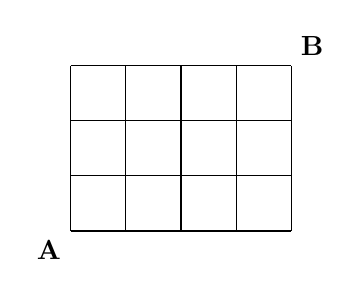
\begin{tikzpicture}[scale=0.7]
                % 縦線を描画(5本の縦線)
                \foreach \x in {0,1,2,3,4}
                    \draw (\x,0) -- (\x,3);

                % 横線を描画(4本の横線)
                \foreach \y in {0,1,2,3}
                    \draw (0,\y) -- (4,\y);

                % Aを左下に配置
                \node[below left] at (0,0) {\textbf{A}};

                % Bを右上に配置
                \node[above right] at (4,3) {\textbf{B}};
            \end{tikzpicture}
        \end{center}
    \end{minipage}
\end{example}

\begin{proof}\mbox{}\\
    交差点から次の交差点に行くのに, ↑ と → の向きがある. このとき, 最短経路は, そのどこを通っても,

    ↑ 3個と → 4個を使って作られる順列に対応している.

    上へ1区画進むことを ↑ で, 右へ1区画進むことを → で表す.
    AからBまで行く最短の道順の総数は, ↑ 3個と → 4個を1列に並べる順列の総数に等しい.

    よって, 求める最短の道順の総数は

    \begin{alignanswer*}
        \dfrac{\,7!\,}{\,3! 4!\,} &= \dfrac{\,7 \cdot 6 \cdot 5 \cdot 4 \cdot 3 \cdot 2 \cdot 1\,}{\,3 \cdot 2 \cdot 1 \times 4 \cdot 3 \cdot 2 \cdot 1\,} \\
                                &= 35 \quad \text{(通り)}
    \end{alignanswer*}
    \vspace{-4\baselineskip}%  この証明環境の空行を減らす
\end{proof}
\newpage

% 練習30
\begin{exercise}[【教p.39 練習30】]
    \begin{minipage}{0.6\textwidth}
        右の図のような道のある地域で, 次のような最短の道順は何通りあるか.
        \begin{enumerate}
            \item AからBまで行く.
            \item AからCを通ってBまで行く.
            \item AからCを通らずにBまで行く.
        \end{enumerate}
    \end{minipage}
    \hfill
    \begin{minipage}{0.35\textwidth}
        \begin{center}
            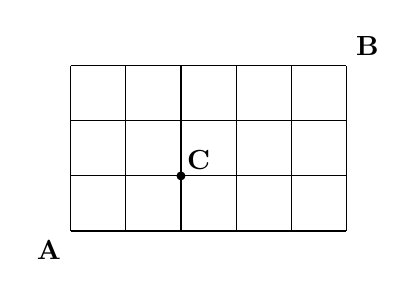
\begin{tikzpicture}[scale=0.7]
                % 縦線を描画(6本の縦線:縦3マス、横5マス)
                \foreach \x in {0,1,2,3,4,5}
                    \draw (\x,0) -- (\x,3);

                % 横線を描画(4本の横線)
                \foreach \y in {0,1,2,3}
                    \draw (0,\y) -- (5,\y);

                % Aを左下に配置
                \node[below left] at (0,0) {\textbf{A}};

                % Bを右上に配置
                \node[above right] at (5,3) {\textbf{B}};

                % Cを座標(2,1)に配置(点を表示し、文字を線と被らないように配置)
                \filldraw[black] (2,1) circle (2pt);
                \node[above right, inner sep=2pt] at (2,1) {\textbf{C}};
            \end{tikzpicture}
        \end{center}
    \end{minipage}
\end{exercise}
\vspace{-1em}%  練習問題環境後の空行を減らす

    \begin{proof}\mbox{}\\
        (1)
        \begin{alignanswer*}
            \dfrac{\,8!\,}{\,3!5!\,} &= \dfrac{\,8 \cdot 7 \cdot 6 \cdot 5 \cdot 4 \cdot 3 \cdot 2 \cdot 1\,}
            {\,3 \cdot 2 \cdot 1 \times 5 \cdot 4 \cdot 3 \cdot 2 \cdot 1\,} \\
                                &= 56 \quad \text{(通り)}
        \end{alignanswer*}
        \vspace{-4\baselineskip}%  この証明環境の空行を減らす
        \end{proof}
    \vspace{-0.5em}%  証明環境間の空行を減らす

    \begin{proof}\mbox{}\\
        (2)
        \begin{alignanswer*}
            \dfrac{\,3!\,}{\,2!1!\,} \times \dfrac{\,5!\,}{\,3!2!\,} &= \dfrac{\,3 \cdot 2 \cdot 1\,}
            {\,2 \cdot 1 \times 1\,} \times \dfrac{\,5 \cdot 4 \cdot 3 \cdot 2 \cdot 1\,}{\,3 \cdot 2 \cdot 1 \times 2 \cdot 1\,} \\
                                &= 30 \quad \text{(通り)}
        \end{alignanswer*}
        \vspace{-4\baselineskip}%  この証明環境の空行を減らす
    \end{proof}
    \vspace{-0.5em}%  証明環境間の空行を減らす

    \begin{proof}\mbox{}\\
        (3)
        \begin{alignanswer*}
            56 - 30 = 26 \quad \text{(通り)}
        \end{alignanswer*}
        \vspace{-4\baselineskip}%  この証明環境の空行を減らす
    \end{proof}
\newpage
